\chapter{Requirements}
\section{Requirements of objective}
\subsection{Asparagus sprout specification \& analysis}
Picking asparagus using a robotic arm involves several steps to ensure proper handling and minimize damage to the plant. The robotic arm needs to detect the presence of asparagus plants in the field and accurately locate them. This can be achieved using sensors such as cameras or LiDAR to identify the position and size of the asparagus plants. But first, we need to localize and categorize the asparagus spear.

\begin{figure}
    \centering
    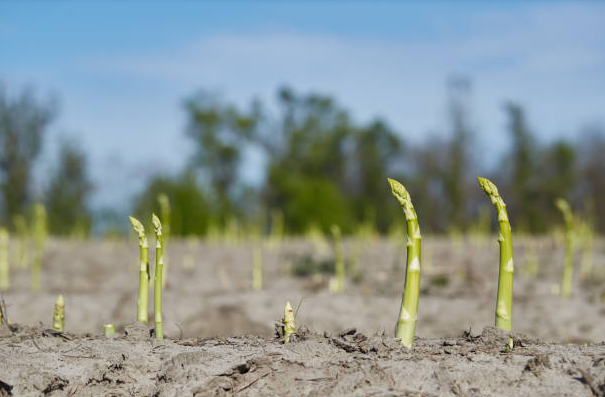
\includegraphics[width=0.75\linewidth]{pictures/asp_in_field.png}
    \caption{asparagus field}
    \label{fig:enter-label}
\end{figure}

Asparagus is a perennial flowering plant species in the genus Asparagus. It is cultivated for its young shoots, which are commonly used as a vegetable. Asparagus can be classified into 4 classes according to the International Standards for Fruit and Vegetables (OECD) \cite{oecd2025}:

1.white asparagus;

2.violet asparagus

3.violet/green asparagus

4.green sprout with slight purple taint

green asparagus having tips and most of the shoot green Our objective is mostly limited to picking the 4th class of asparagus. The asparagus must not have any damage or injury spoiling the integrity of the produce. It has to be practically unbruised and has to have a clean cut. For detection and localization of the target spear, I have followed the standards of OECD.

It is defined according to the length sizing and diameter of a spear, which is given below:
By length:
1.Above 17 cm for long asparagus
2.12 to 17 cm for short asparagus
The maximum length allowed for green asparagus is 27 cm.
\begin{figure}
    \centering
    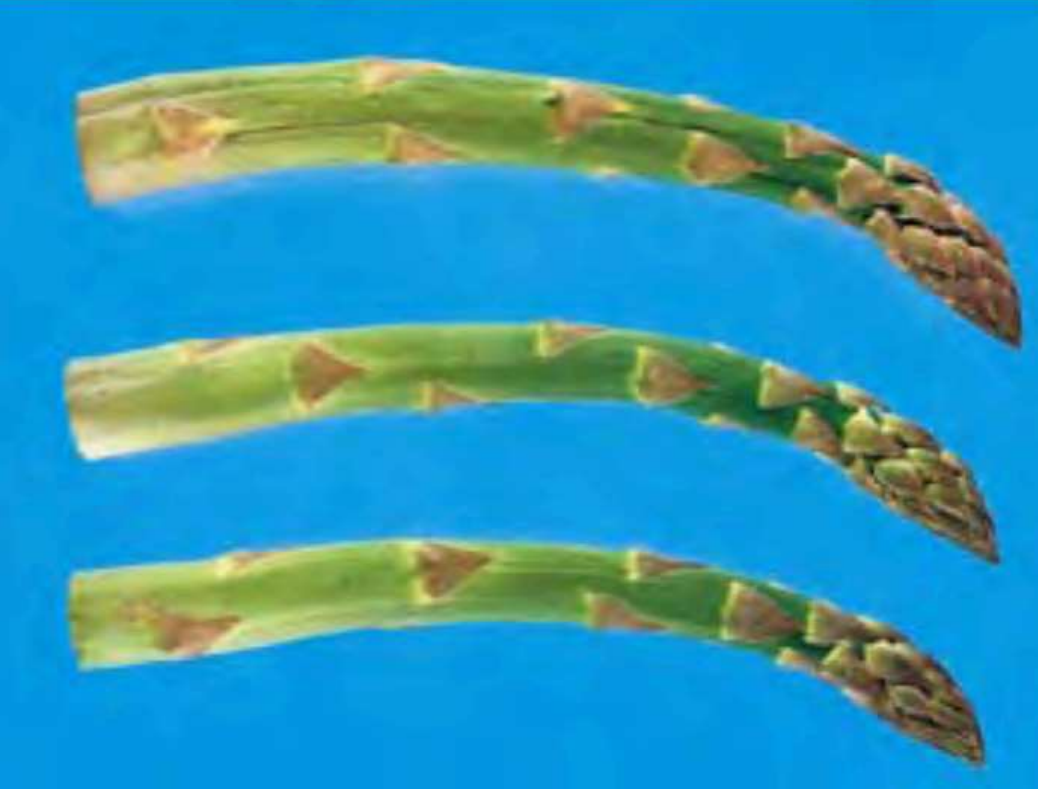
\includegraphics[width=0.75\linewidth]{pictures/class_1_limitedbending.png}
    \caption{class 1 harvest}
    \label{fig:enter-label}
\end{figure}
\begin{figure}
    \centering
    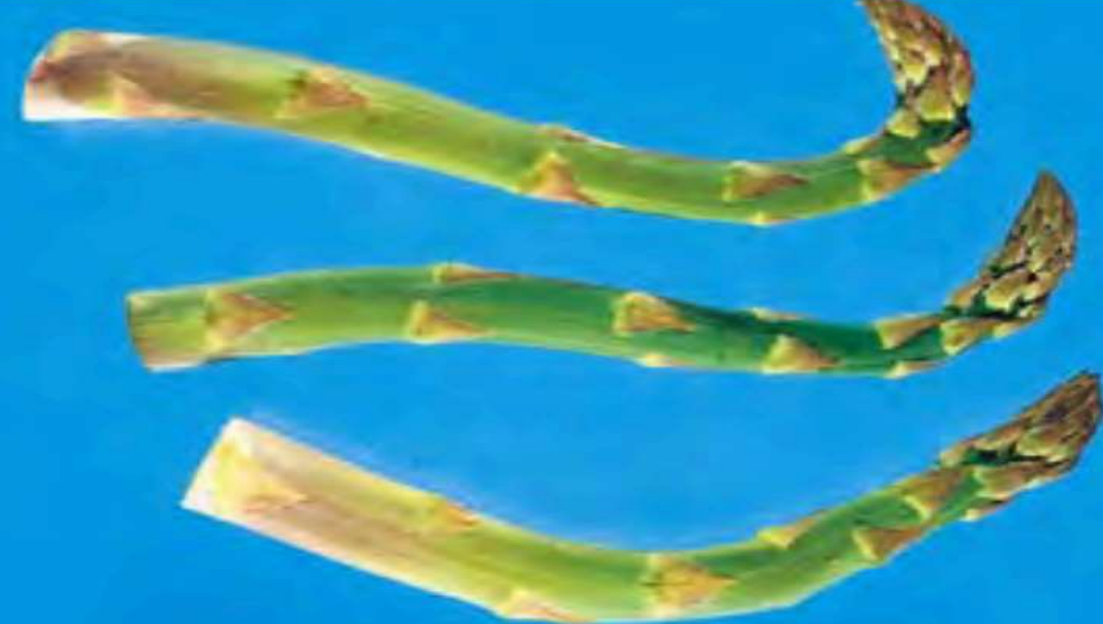
\includegraphics[width=0.75\linewidth]{pictures/class2_superier_bending.png}
    \caption{class 2 harvest}
    \label{fig:enter-label}
\end{figure}

By diameter:

1.Class I should have a minimum 3 mm diameter to a maximum of 8 mm.

2.Class II should have 3 mm with no range of uniformity in the bundle.

For all classes, asparagus must comply with a minimum 
diameter in accordance with the relevant group.

\section{Proposed Robotic Arm Design}
The proposed robotic arm, tailored for asparagus 
harvesting, is a meticulously engineered solution 
designed to integrate AI-driven computer vision  with a lightweight, 
durable mechanical structure to address labor 
shortages, enhance precision, and promote sustainable 
farming practices. For simplicity and experimentation 
in lab condition, I have decided to start with a 3DoF 
RRR robot arm. A hand drawn illustration is given below 
in the following figure 2.4.




\begin{figure}[H]
    \centering
    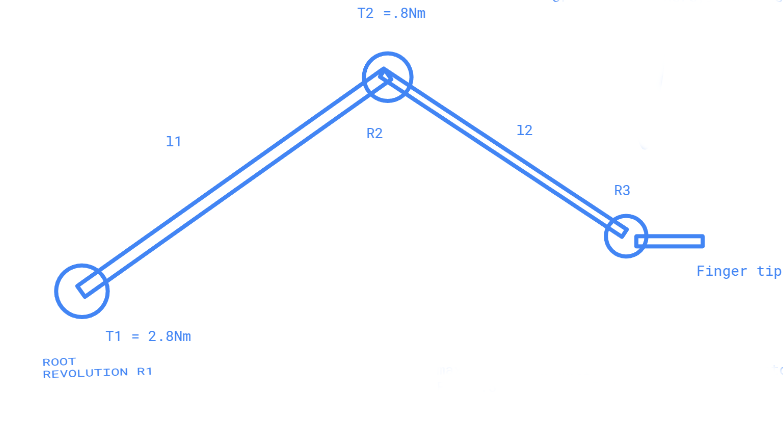
\includegraphics[width=1\linewidth]{pictures/robot_illustration.png}
    \caption{hand drawn illustration of the planned robot arm}
    \label{fig:enter-label}
\end{figure}


Designing an RRR (Revolute-Revolute-Revolute) robotic arm for asparagus harvesting requires careful consideration of mechanical, kinematic, and operational requirements to ensure efficient, precise, and sustainable harvesting in challenging field conditions. The primary design requirement is structural stability to handle the dynamic loads during operation, as the arm must support torques . This necessitates robust motors, such as NEMA 17 with a sufficient rated torque, and a servo gear reduction ratio to provide sufficient power while maintaining control. Reach and precision are critical, given asparagus spears’ low-lying growth (10-30 cm above ground); the arm’s links, L1  and L2 , must achieve a total reach of at least 0.45 m (considered lab condition), with degrees of freedom (DOF) of allowing precise positioning within a 0 to 90-degree range for L1 and 0 to 120-degree range for L2. Lightweight construction is essential to minimize energy consumption and soil compaction using materials like aluminum or wood for the links. Durability in harsh field conditions---such as dust, moisture, and temperature variations (0--40$^\circ$C)---requires weather-resistant coatings and sealed joints to protect motors and electronics. Integration with computer vision, such as the Mask R-CNN model implemented, demands a mounting point for a multi-spectral camera and an edge device (e.g., NVIDIA Jetson Xavier NX) to process detection and segmentation data in real-time, under 0.5 seconds per frame, aligning with the arm’s velocity . Energy efficiency is a key consideration, as the arm must operate for 8--10 hours on a portable battery, potentially supplemented by solar panels, to support the computational demands of AI systems. Cost-effectiveness is crucial for adoption by small-scale farmers, aiming for a production cost below \$5,000 through modular design and off-the-shelf components like NEMA 17 motors. Ease of maintenance is also vital, incorporating a modular structure for quick joint replacement and a design that allows farmers to perform basic repairs without specialized tools. Additionally, the arm must minimize environmental impact by avoiding excessive soil disturbance and supporting sustainable practices, such as reducing herbicide use through precise weed identification. These requirements and considerations ensure the RRR robotic arm can effectively harvest asparagus, addressing labor shortages while maintaining high yield quality and operational reliability in diverse agricultural settings.In the following table we provide a minimum requirements for my proposed solution


\begin{table}[h!]
\centering
\caption{proposed Key Design requirements of the Robotic Arm for Asparagus Harvesting}
\label{tab:robotic_arm_specs}
\begin{tabular}{|l|l|}
\hline
\textbf{Parameter} & \textbf{Value} \\ \hline
Expected workspace dimension & .5 m X .5 m \\ \hline
Servo Gear Reduction Ratio & 30/1 \\ \hline
Motor Type & NEMA 17 \\ \hline
Motor Weight & 0.3 kg \\ \hline
Rated Torque (Motor) & .4 Nm \\ \hline
Torque at Joint R1 (T1) & 3.36 Nm \\ \hline
Torque at Joint R2 (T2) & .8 Nm \\ \hline
Maximum Torque (Fully Stretched) & 3.36 Nm (with 30\% margin) \\ \hline
Total Weight at Joint R2 & 0.46 kg (0.3 kg motor + 0.16 kg components) \\ \hline
Total Weight at Joint R3 & 0.3 kg \\ \hline
Degrees of Freedom (DOF) & RRR \\ \hline
Link Length (l1) & 0.25 m \\ \hline
Link Length (l2) & 0.2 m \\ \hline
Material &  aluminum  and PLA plastic\\ \hline
\end{tabular}
\end{table}









\section{Requirements for Computer Vision:Asparagus Detection and Segmentation }


Selecting a computer vision model for asparagus detection and segmentation requires balancing multiple criteria to ensure the robotic arm can efficiently and accurately harvest spears in dynamic field conditions. The primary priority is real-time performance, as the system must process frames in under 0.5 seconds to enable rapid picking, aligning with the arm’s velocity .asparagus harvesting demands both detection and precise segmentation to isolate spears from weeds. The image processing model should also be the backbone that should  provides robust feature extraction, essential for distinguishing asparagus spears in cluttered environments with shadows and varying lighting. Accuracy is the second priority, as false positives or missed spears could damage crowns or reduce yield. Resource efficiency is critical due to the edge deployment on the robotic arm since the model's comprehensive output with workload should justifies the computational cost, especially with the Jetson’s (Jetson Xavier NX)21 TOPS capacity. Adaptability to field variations (e.g., spear size, occlusion by weeds) is another key factor. Ease of integration with the robotic arm via ROS is also considered which offers seamless ROS integration through pre-built pipelines, outputting bounding boxes and masks directly usable by the arm’s control system. 


